\section{Semaine 14 : 08/05/2023 - 12/05/2023}
\graphicspath{{semaines/semaine_14/images/}}

\begin{abstract}
	Après discussion avec Emmanuel, il semblerait que les résultats obtenus pour $\tilde{\phi}$ de degré 2 ne soient pas aberrant. On va alors continuer les tests sur le FNO avec la deuxième méthode et comparer la résultats avec PhiFEM et FEM.  On va également tester de faire une IPP sur le second membre $\tilde{f}$ pour n'utiliser que les dérivées premières de $\tilde{\phi}$. On comparera les résultats avec et sans IPP.

	Dans un second temps, on souhaite faire fonctionner le rehaussemen avec PhiFEM en utilisant la méthode duale. On commencera par faire les courbes de convergence puis on essayera de faire les mêmes comparaisons que pour FEM entre la première méthode de correction avec et sans rehaussement et la seconde.
	
	Vanessa a également proposée une nouvelle idée qui consiste à combiner les deux méthodes de correction, en posant quelque chose comme $\tilde{f}=\hat{\phi}C_1+C_2$. On fera la théorie dessus et on testera numériquement lorsque les idées précédentes seront faites.
\end{abstract}

\subsection{2ème méthode de Correction}

\subsection{Méthode duale}

On considère le problème de Poisson avec condition de Dirichlet homogène ou non homogène :
\begin{equation*}
	\left\{\begin{aligned}
		&-\Delta u=f \quad &&\Omega \\
		&u=g \quad &&\Gamma
	\end{aligned}\right.
\end{equation*}

La formulation variationnelle PhiFEM pour ce problème en utilisant la méthode duale est :

$$\int_{\Omega_h}\nabla u\nabla v-\int_{\partial\Omega_h}\frac{\partial u}{\partial n} v + \frac{\gamma}{h^2} \sum_{T\in\mathcal{T}_h^\Gamma}\int_T \left(u-\frac{1}{h}\phi p\right)\left(v-\frac{1}{h}\phi q\right) + G_h(u,v) = \int_{\Omega_h}fv + \frac{\gamma}{h^2} \sum_{T\in\mathcal{T}_h^\Gamma}\int_T g\left(v-\frac{1}{h}\phi q\right) + G_h^{rhs}(v)$$
avec
$$G_h(u,v)=\sigma h\sum_{E\in\mathcal{F}_h^\Gamma}\int_E\left[\frac{\partial u}{\partial n}\right]\left[\frac{\partial v}{\partial n}\right]+\sigma h^2\sum_{T\in\mathcal{T}_h^\Gamma}\int_T \Delta u\Delta v$$
et
$$G_h^{rhs}(v)=-\sigma h^2\sum_{T\in\mathcal{T}_h^\Gamma}\int_T f\Delta v$$

Pour la correction, on considère le problème suivant :

\begin{equation*}
	\left\{\begin{aligned}
		&-\Delta (\hat{\phi}C)=f \quad &&\Omega \\
		&\hat{u}=g+m \quad &&\Gamma
	\end{aligned}\right. \label{pbc1r}
\end{equation*}
avec $\hat{u}=\hat{\phi}C+m$ où $\hat{\phi}=\tilde{\phi}+m$ ($m$ une constante).

La formulation variationnelle PhiFEM pour ce problème en utilisant la méthode duale est :
\begin{align*}
	\int_{\Omega_h}\nabla(\hat{\phi}C)\nabla(\hat{\phi}v)-\int_{\partial\Omega_h}\frac{\partial}{\partial n}(\hat{\phi}C)\hat{\phi}v + \frac{\gamma}{h^2} \sum_{T\in\mathcal{T}_h^\Gamma}\int_T \left(\hat{\phi} C-\frac{1}{h}\phi p\right)\left(\hat{\phi}v-\frac{1}{h}\phi q\right) + G_h(C,v)& \\
	= \int_{\Omega_h}f\hat{\phi}v + \frac{\gamma}{h^2} \sum_{T\in\mathcal{T}_h^\Gamma}\int_T (g+m)\left(\hat{\phi}v-\frac{1}{h}\phi q\right) + G_h^{rhs}(v)&
\end{align*}
avec
$$G_h(C,v)=\sigma h\sum_{E\in\mathcal{F}_h^\Gamma}\int_E\left[\frac{\partial}{\partial n}(\hat{\phi}C)\right]\left[\frac{\partial}{\partial n}(\hat{\phi}v)\right]+\sigma h^2\sum_{T\in\mathcal{T}_h^\Gamma}\int_T \Delta(\hat{\phi}C)\Delta(\hat{\phi}v)$$
et
$$G_h^{rhs}(v)=-\sigma h^2\sum_{T\in\mathcal{T}_h^\Gamma}\int_T f\Delta(\hat{\phi}v)$$

\newpage

Voici les résultats obtenus :

\begin{minipage}{0.38\linewidth}
	\centering
	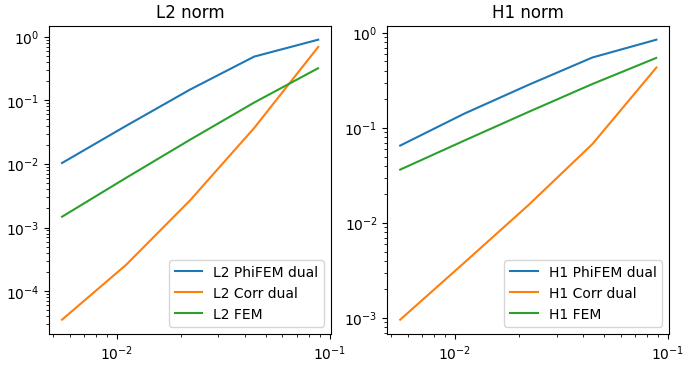
\includegraphics[width=\linewidth]{dual_courbes.png}
\end{minipage}
\begin{minipage}{0.58\linewidth}
	\centering
	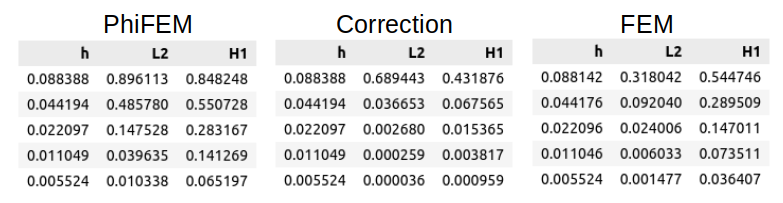
\includegraphics[width=\linewidth]{dual_results.png}
\end{minipage}